\chapter{Hauptcharaktere}
\section{Soldat} \label{sec:mc-soldat}
\begin{outline}
	\1 männlich
	\1 Alter:
		\2 16 Jahre während Demo
	\1 Aussehen:
		\2 dargestellt in Abb. \ref{fig:mc-soldat}
		\2 rötliche Haare, bis zu den Augenbrauen
		\2 Sommersprossen
		\2 sonnengebrannte Haut
		\2 strammer Typ
	\1 Kleidung:
		\2 praktikabel
		\2 mit etwas Schutz
	\1 Charakter:
		\2 bodenständig 
		\2 optimistisch 
		\2 charmant 
	\1 Abstammung:
		\2 Vater: hochdekorierter Militär, nie Zuhause. War mal im Dorf stationiert -> dadurch mit Mutti zusammen gekommen
		\2 Mutter: stammt aus dem Dorf, liebevolle Beziehung
		\2 Geschwister: mind. 1 offen
	\1 Hintergrund:
		\2 aufgewachsen im Kerndorf
		\2 hohes Interesse an den stationierten Soldaten, verbringt Freizeit auch gerne bei denen
		\2 eifert seinem Vater nach, will aus dem Dorf raus
		\2 eher wohlhabend
\end{outline}

\begin{figure}[tbh]
	\centering
	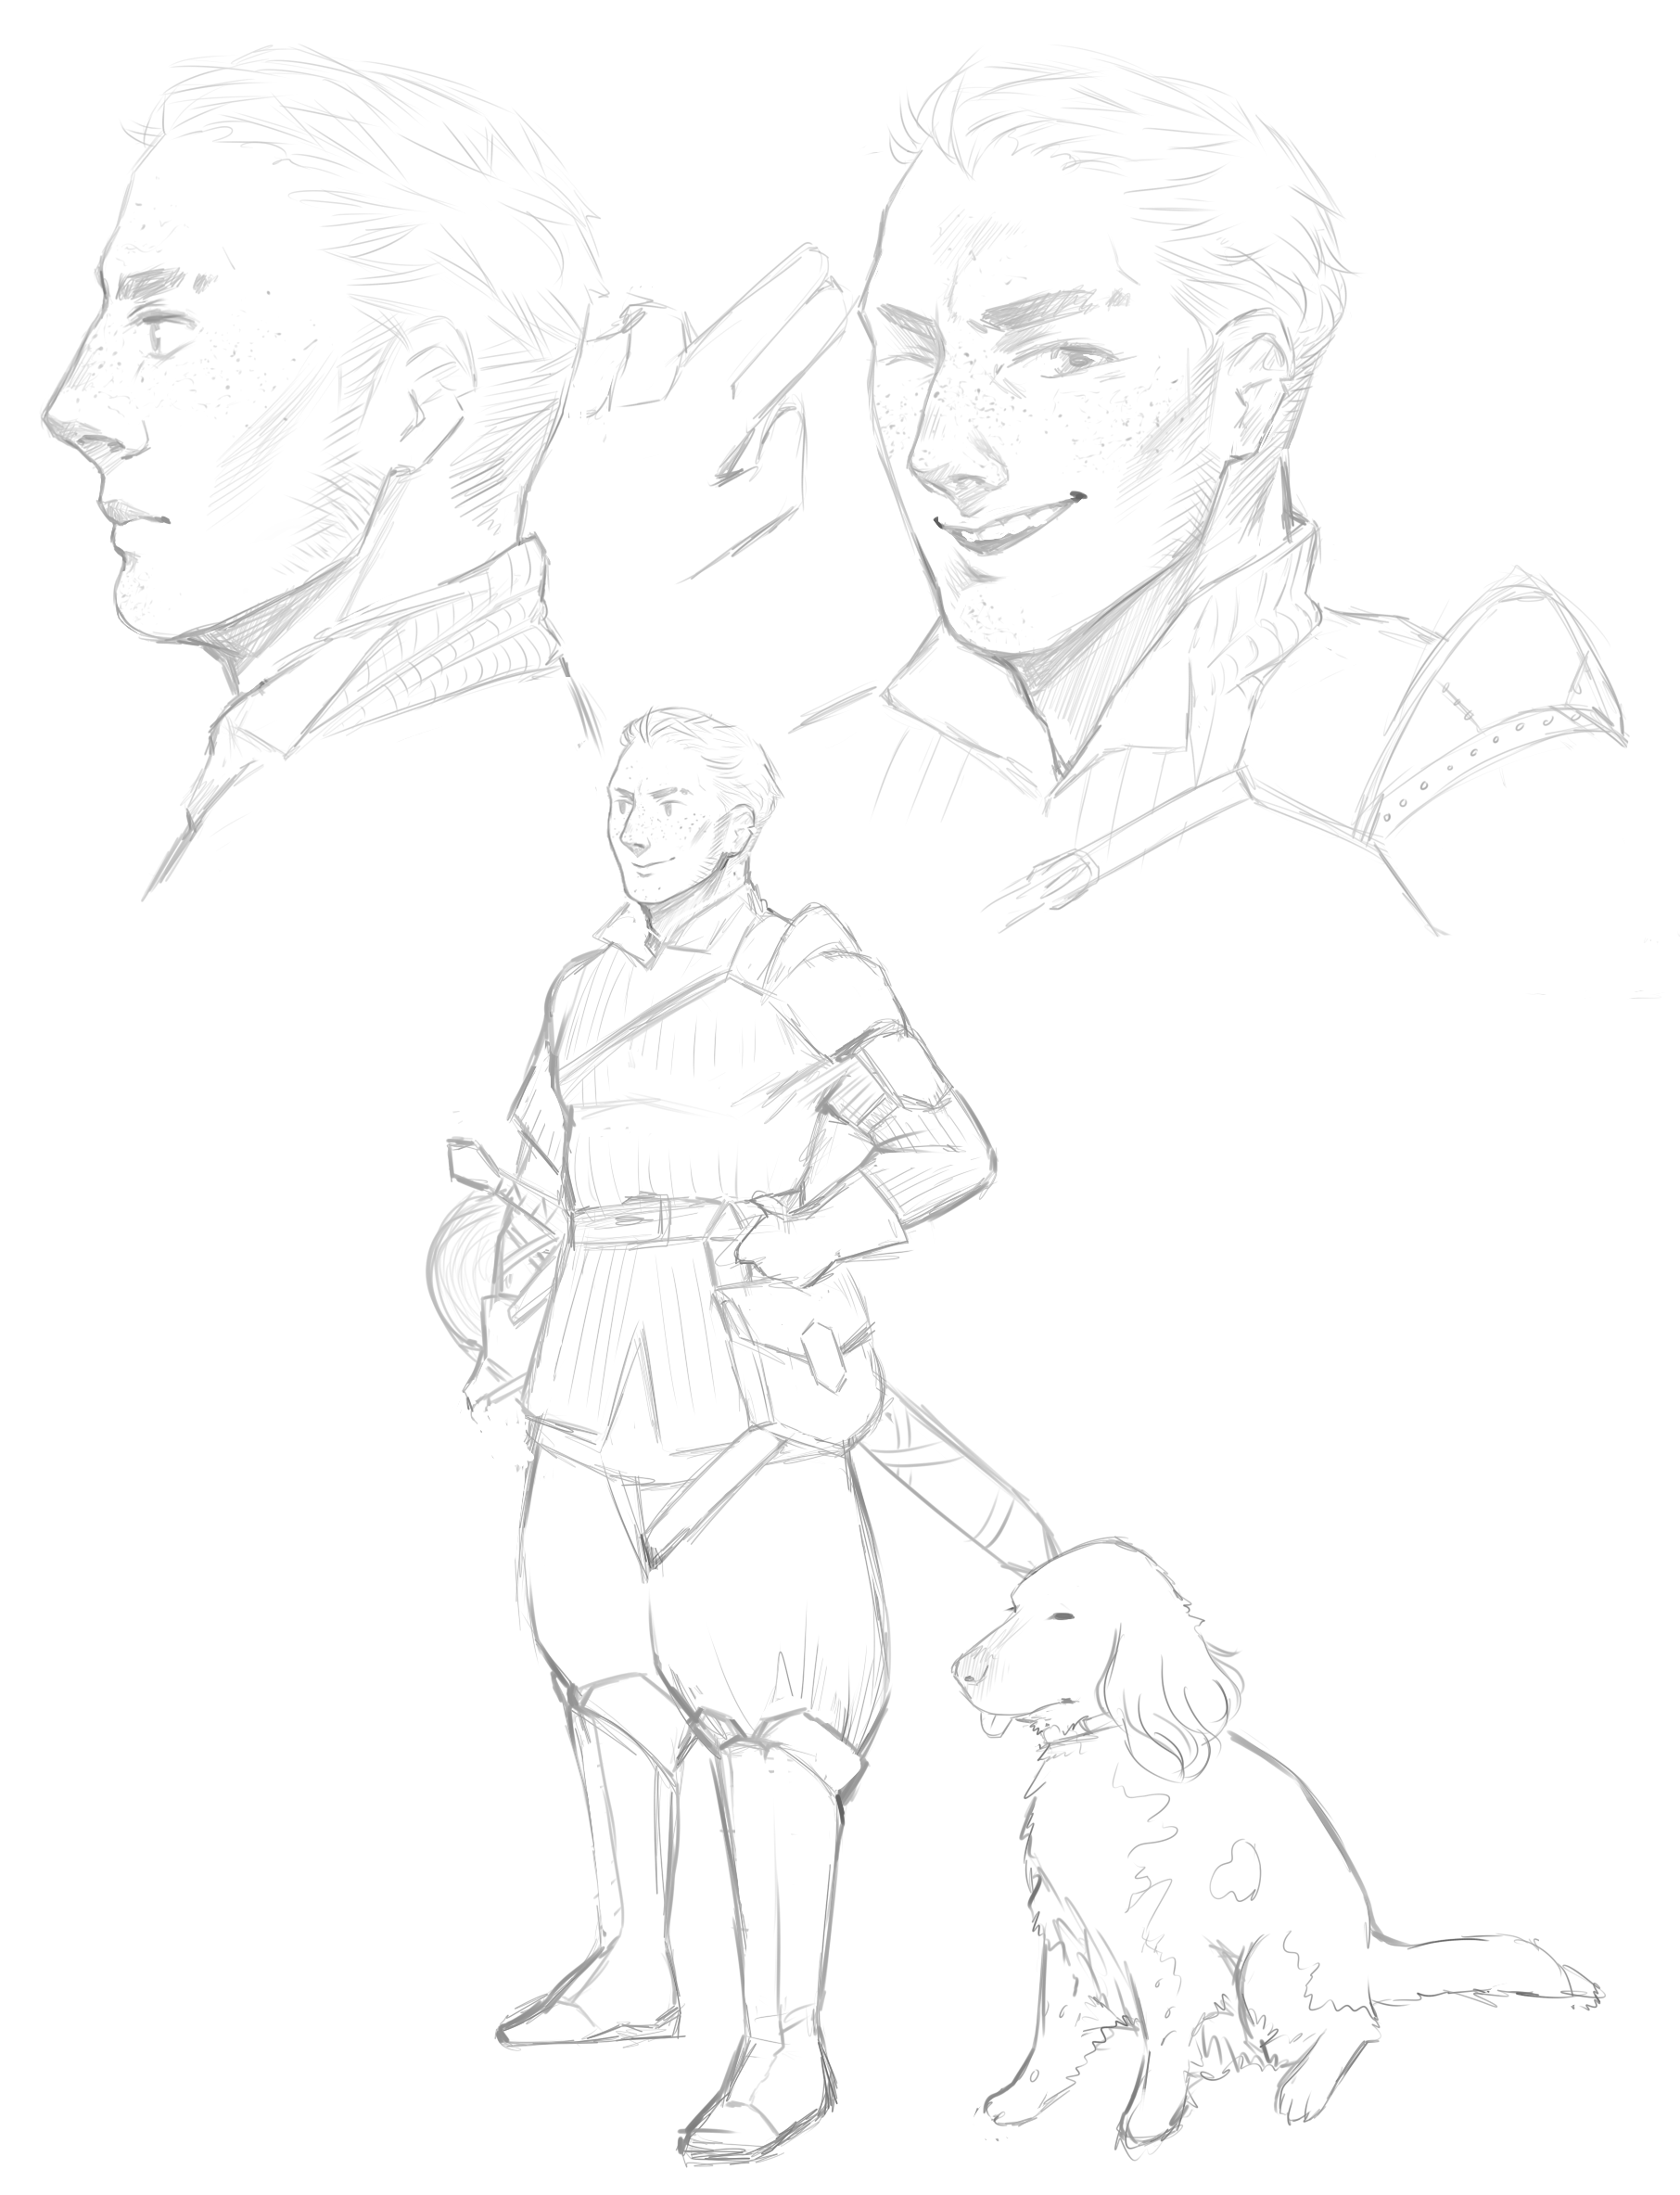
\includegraphics[width=0.75\textheight]{Abbildungen/Abenteuer/Hauptcharaktere/soldat.png}
	\caption[Konzeptart Soldat]{Konzeptart Soldat als 16-Jähriger während dem Hauptteil der Demo.}
	\label{fig:mc-soldat}
\end{figure}

\section{Diplomatin} \label{sec:mc-diplomatin}
\begin{outline}
	\1 weiblich
	\1 Alter:
		\2 17 zur Demo
	\1 Aussehen:
		\2 wie dargestellt in Abb. \ref{fig:mc-diplomatin} 
		\2 gut gepflegt 
		\2 geschminkt
	\1 Kleidung:
		\2 legt Wert auf Äußeres
		\2 lange Kleider
	\1 Charakter:
		\2 "Mädchen"
		\2 ihr ist die Ehre der Familie sehr wichtig 
		\2 legt viel Wert darauf, was andere von ihr halten 
		\2 sehr offen gegenüber den schlechter beglückten
	\1 Abstammung:
		\2 Mutter: die Geistliche im Amt, eingereist
		\2 Vater: deren Mann, Städter, musste mit seiner Frau mit. Während der Char ein Kind ist, ist er noch sehr unglücklich, später hat er sich mit einigen Männern angefreundet und sich mit der Situation zurechtgefunden. Arbeitet bei einem der innerdörflichen Berufe mit
		\2 Geschwister: mind. 3 offen
	\1 Hintergrund:
		\2 absolut gläubig erzogen
		\2 eifert ihrer Mutter darin nach, eine hohe Position im Orden zu erlangen und diesem weiter zu helfen
\end{outline}

\begin{figure}[tbh]
	\centering
	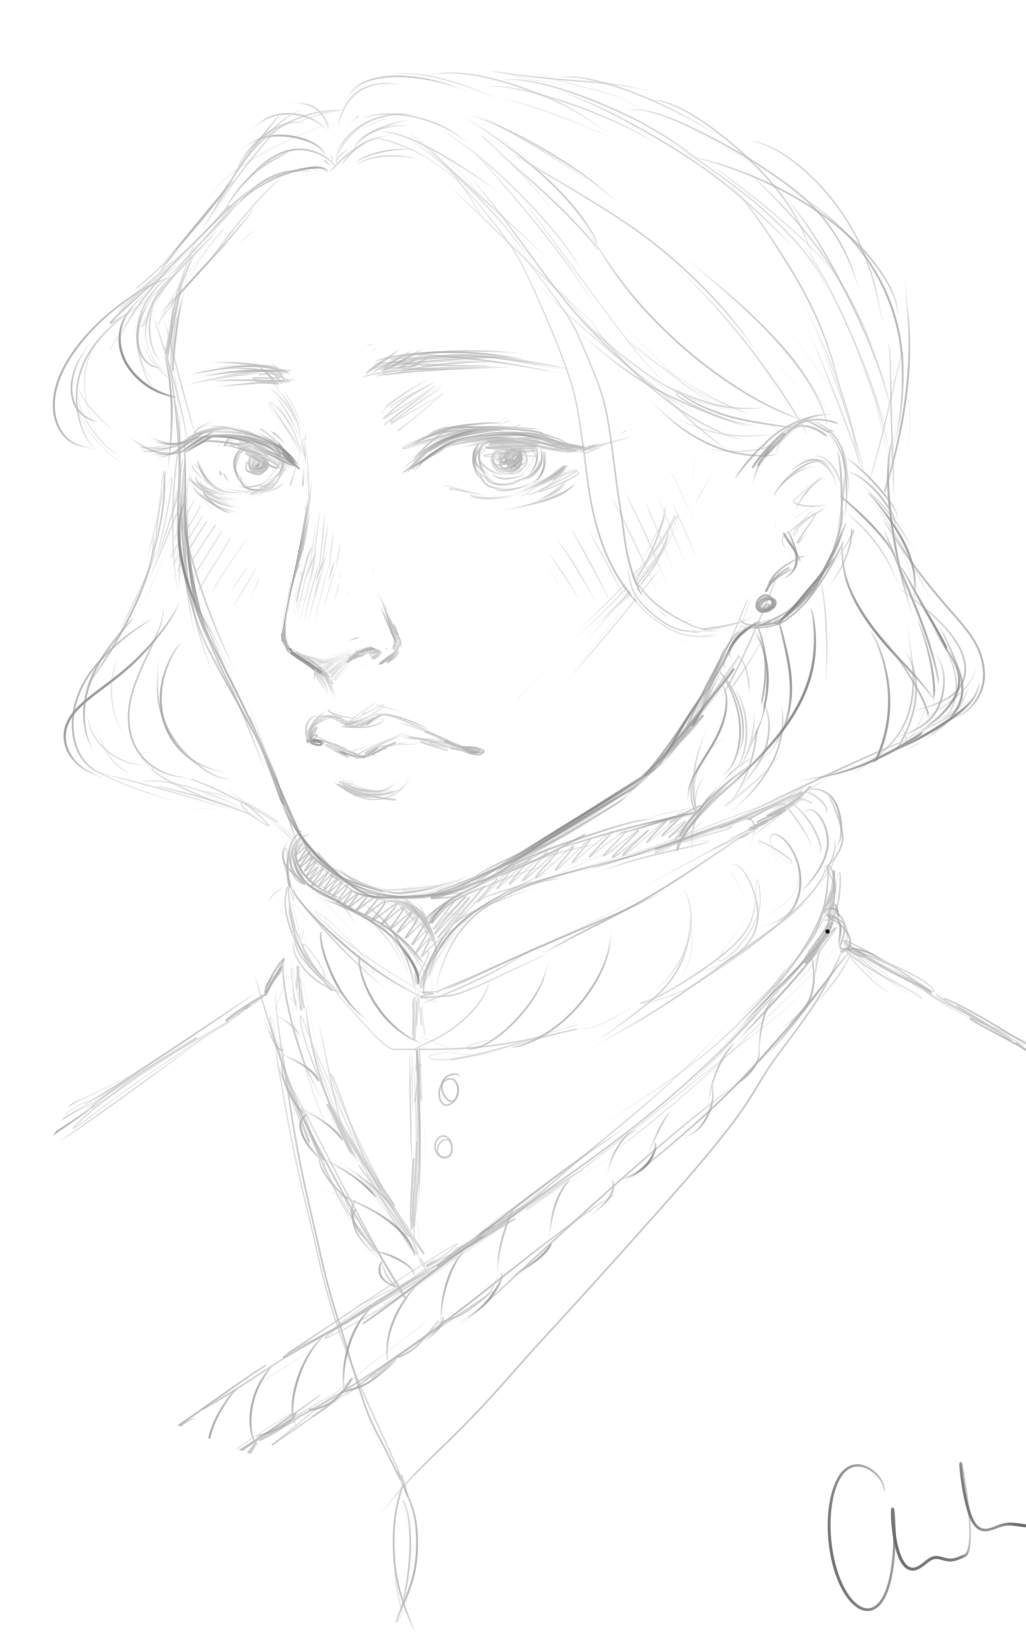
\includegraphics[width=0.325\textheight]{Abbildungen/Abenteuer/Hauptcharaktere/magierin}
	\caption[Konzeptart Diplomatin]{Konzeptart Diplomatin als 17-Jährige während dem Hauptteil der Demo.}
	\label{fig:mc-diplomatin}
\end{figure}


\section{Spionin} \label{sec:mc-spionin}
\begin{outline}
	\1 weiblich
	\1 Alter:
		\2 16 zur Demo
	\1 Aussehen:
		\2 wie dargestellt in Abb. \ref{fig:mc-spionin}
		\2 Zopf bis Brust
	\1 Kleidung:
		\2 praktisch
		\2 Hosen 
		\2 Bogen, Dolch (zum Ausnehmen Wild) am Gürtel
		\2 Gugel?
	\1 Charakter:
		\2 praktisch veranlagt
		\2 Wildfang 
		\2 zynisch 
		\2 schwarzer Humor
	\1 Abstammung:
		\2 Vater: Jäger
		\2 Mutter: 
		\2 Geschwister: einige offen
	\1 Hintergrund:
		\2 arme und ungebildete Familie
		\2 aufgewachsen am Rand des Dorfes oder ggf. am Waldrand bei den 2-3 Jägerhütten
\end{outline}

\begin{figure}[tbh]
	\centering
	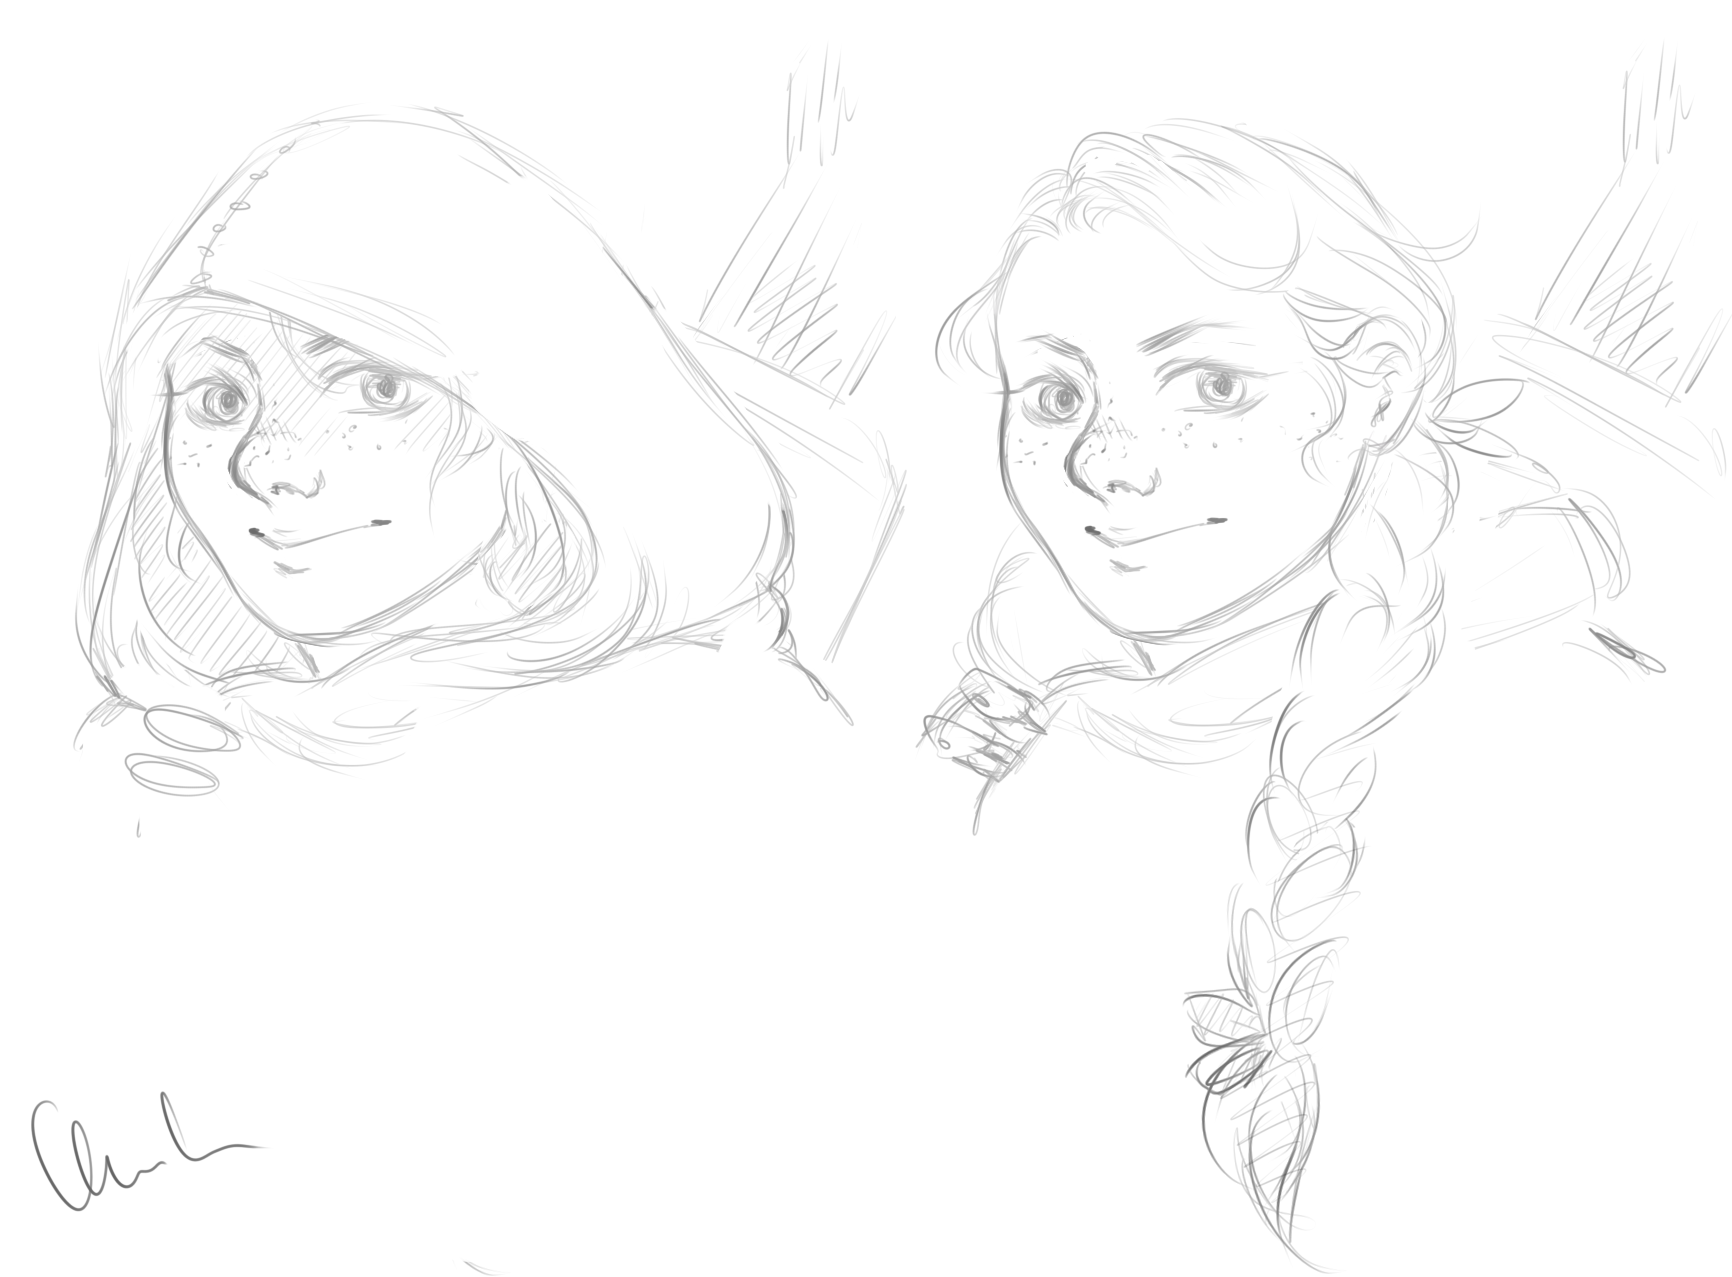
\includegraphics[width=0.9\textwidth]{Abbildungen/Abenteuer/Hauptcharaktere/spionin}
	\caption[Konzeptart Spionin]{Konzeptart Spionin als 16-Jährige während dem Hauptteil der Demo.}
	\label{fig:mc-spionin}
\end{figure}
